% Pandoc template for Physical Review D (REVTeX 4.2, preprint/one-column).
% Retargeted from MNRAS: MNRAS became fully open access in 2024 with a mandatory
% APC (GBP 2,356), and no APC waiver is being sought. PRD is free on the
% subscription route. Engine: pdflatex (REVTeX is pdflatex-native).
\documentclass[aps,prd,preprint,nofootinbib,superscriptaddress]{revtex4-2}
\usepackage{iftex}
\ifPDFTeX
  \usepackage[T1]{fontenc}
  \usepackage[utf8]{inputenc}
\else
  \usepackage{fontspec}
  \setmainfont{STIX Two Text}
\fi

\usepackage{amsmath,amssymb,graphicx}
\usepackage[hidelinks]{hyperref}
\usepackage{orcidlink}

\makeatletter
\let\pandocsurd\surd \renewcommand{\surd}{\ensuremath{\pandocsurd}}
\makeatother
\hyphenation{zenodo Zenodo}
% pdflatex needs this explicitly; xelatex+STIX had it for free
\usepackage{newunicodechar}
\newunicodechar{ℏ}{\ensuremath{\hbar}}
\providecommand{\eprint}[1]{#1}
\AtBeginDocument{\renewcommand{\eprint}[1]{\href{https://arxiv.org/abs/#1}{#1}}}

% --- prose Unicode operators -> math (works under xe/pdf latex) ---
\usepackage{newunicodechar}
\newunicodechar{→}{\ensuremath{\rightarrow}}
\newunicodechar{∂}{\ensuremath{\partial}}
\newunicodechar{∈}{\ensuremath{\in}}
\newunicodechar{∎}{\ensuremath{\blacksquare}}
\newunicodechar{□}{\ensuremath{\Box}}
\newunicodechar{∝}{\ensuremath{\propto}}
\newunicodechar{∞}{\ensuremath{\infty}}
\newunicodechar{∫}{\ensuremath{\int}}
\newunicodechar{≈}{\ensuremath{\approx}}
\newunicodechar{≠}{\ensuremath{\neq}}
\newunicodechar{≡}{\ensuremath{\equiv}}
\newunicodechar{≤}{\ensuremath{\leq}}
\newunicodechar{≥}{\ensuremath{\geq}}
\newunicodechar{≪}{\ensuremath{\ll}}
\newunicodechar{≫}{\ensuremath{\gg}}
\newunicodechar{≲}{\ensuremath{\lesssim}}
\newunicodechar{⊙}{\ensuremath{\odot}}
\newunicodechar{⊗}{\ensuremath{\otimes}}
\newunicodechar{⟹}{\ensuremath{\Longrightarrow}}
\newunicodechar{⟺}{\ensuremath{\Longleftrightarrow}}
\newunicodechar{⇒}{\ensuremath{\Rightarrow}}
\newunicodechar{⇔}{\ensuremath{\Leftrightarrow}}
\newunicodechar{𝓗}{\ensuremath{\mathcal{H}}}
\newunicodechar{√}{\ensuremath{\surd}}
\newunicodechar{∼}{\ensuremath{\sim}}
\newunicodechar{∇}{\ensuremath{\nabla}}
\newunicodechar{↔}{\ensuremath{\leftrightarrow}}
\newunicodechar{⟨}{\ensuremath{\langle}}
\newunicodechar{⟩}{\ensuremath{\rangle}}
\newunicodechar{−}{\ensuremath{-}}
\newunicodechar{ℓ}{\ensuremath{\ell}}
\newunicodechar{ħ}{\ensuremath{\hbar}}
\newunicodechar{′}{\ensuremath{{}^\prime}}
\newunicodechar{Ḣ}{\ensuremath{\dot H}}
\newunicodechar{Ṡ}{\ensuremath{\dot S}}
\newunicodechar{₊}{\ensuremath{{}_{+}}}

% --- pandoc body requirements ---
\usepackage{longtable,booktabs,array}
\usepackage{calc}
\usepackage{float}
\makeatletter
\newsavebox\pandoc@box
\newcommand*\pandocbounded[1]{%
  \sbox\pandoc@box{#1}%
  \Gscale@div\@tempa{\textheight}{\dimexpr\ht\pandoc@box+\dp\pandoc@box\relax}%
  \Gscale@div\@tempb{\linewidth}{\wd\pandoc@box}%
  \ifdim\@tempb\p@<\@tempa\p@\let\@tempa\@tempb\fi%
  \ifdim\@tempa\p@<\p@\scalebox{\@tempa}{\usebox\pandoc@box}%
  \else\usebox{\pandoc@box}%
  \fi%
}
\makeatother
\providecommand{\tightlist}{\setlength{\itemsep}{0pt}\setlength{\parskip}{0pt}}
\graphicspath{{../}{../figures/}}

\setlength{\emergencystretch}{6em}
\sloppy

\begin{document}

\title{The Galactic Face of the Entropy Clock: MOND as a Rate-Branch
Acceleration Scale a\(_{0}\) \(\propto\) H(z)}

\author{Stilian Pandev\,\orcidlink{0009-0005-8153-071X}}
\email{stilianpandev@gmail.com}
\affiliation{Independent researcher}

\begin{abstract}
The MOND acceleration scale a\(_{0}\) \(\approx\) 1.2 × 10\(^{-10}\) m
s\(^{-2}\) sits, coincidentally, at cH\(_{0}\)/2\(\pi\). We ask whether
this is a coincidence or the galactic readout of the same
horizon-entropy clock that, in the USC program, drives dark energy
(dusk) and matter genesis (dawn). Two cosmological completions of the
coincidence are possible: a \textbf{density branch} a\(_{0}\)
\(\propto\) \(\sqrt{\rho_{\rm DE}}\) (falling with redshift), realized
by the APDM superfluid, and a \textbf{rate branch} a\(_{0}\) \(\propto\)
H(z) (rising), realized by horizon-entropic / emergent gravity. This
rate-vs-density discrimination is not new --- it was posed by
\citep{Limbach:2008aa} (2008), who reached the marginally
\emph{opposite} (density-favoured) verdict. Against the MUSE-DARK III
measurement a\(_{0}\)(z) = (1.00 \(\pm\) 0.04) + (1.59 \(\pm\) 0.11)z
(ratio 2.16 \(\pm\) 0.06 over z = 0.33 \(\to\) 1.44), the density branch
is \textbf{excluded at +16.7\(\sigma\)} (from matching the MUSE-DARK III
fit) --- it predicts a \emph{fall}, the data \emph{rise}: a
\textbf{wrong-sign} miss that is robust to the modeling chain and
therefore fatal. The rate branch matches the \emph{sign} but is
\textbf{amplitude-short at +4.4\(\sigma\)} --- an offset that, unlike a
sign error, is absorbable into the same modeling systematics; the rate
branch is thus \emph{disfavoured but not sign-excluded}, not a clean
survivor. We are explicit that these two verdicts are held to different
standards \emph{by design} --- sign is modeling-robust, amplitude is
not. We flag prominently that this significance is \textbf{conditional
on the MUSE modeling chain}: the rise is not merely unconfirmed but
\emph{absent --- indeed reversed} (\(\beta\) \(\approx\) -0.38) in the
raw released kinematics, which remains an open question. We then locate
the surviving branch: we derive that the ECCG dark-sector scalar is too
short-range by 10\(^{33}\) to carry MOND, and a gated-Verlinde elastic
MOND is excluded inside USC at 19--27\(\sigma\) (from matching the same
data); the unique survivor is a \textbf{KMS-tilt modified inertia} whose
zero-freedom interpolation passes the RAR at 0.057 dex (again a match to
the empirical relation). A worldline influence-functional calculation
derives the acceleration-selective coupling structure and a closed-form
kernel (a/4\(\pi\))cot(\(\pi\)a/\(\kappa\)) in which the conjectured
Green-function 4\(\pi\) genuinely appears (derived in a proxy model),
but not yet the full a\(_{0}\) coefficient, which remains open. The
coefficient-independent, pre-registered prediction is a\(_{0}\)(z)
\(\propto\) H(z) with \textbf{no saturation gate} --- MOND
\emph{strengthens} at high z (a\(_{0}\)(3)/a\(_{0}\)(0) \(\approx\) 4.5
while \(\Omega\)\_DE(z=3) \(\approx\) 3\%) --- falsifiable by JWST
high-z rotators, though existing declining high-z rotation curves
already disfavour a strongly rising a\(_{0}\) \citep{Milgrom:2017hpv}:
the central tension this branch must survive.
\end{abstract}

\maketitle

\noindent\textbf{Keywords:} modified Newtonian dynamics; galaxy rotation
curves; dark energy; emergent gravity; radial acceleration relation
\vspace{6pt}

\section{Introduction}\label{sec-1}

Milgrom's modified dynamics (MOND) \citep{Milgrom:1983ca, Famaey:2011kh}
organizes an enormous body of galactic phenomenology --- the baryonic
Tully--Fisher relation, the radial acceleration relation (RAR), the
mass-discrepancy--acceleration relation --- around a single acceleration
scale a\(_{0}\) \(\approx\) 1.2 × 10\(^{-10}\) m s\(^{-2}\). Below
a\(_{0}\) the dynamics depart from Newton; above it they return. The
empirical tightness of the RAR (scatter \(\lesssim\) 0.13 dex)
\citep{McGaugh:2016leg, Lelli:2016cui} is the strongest evidence that
a\(_{0}\) is a genuine physical scale, not a fitting convenience.

The number a\(_{0}\) is numerically close to cH\(_{0}\)/2\(\pi\). This
coincidence --- a \emph{galactic} acceleration equal to a
\emph{cosmological} rate times a bare 2\(\pi\) --- has been noted since
Milgrom's original papers \citep{Milgrom:2020cch} and is the germ of
every attempt to tie a\(_{0}\) to cosmology. If it is not an accident,
then a\(_{0}\) inherits a time dependence from the cosmological quantity
it tracks, and galaxies at high redshift become a cosmological probe.

This is Paper VIII of the USC program (the program map is set out in the
companion USC program map). USC posits a single \textbf{entropy clock}
--- the horizon entropy-production rate, encoded by \(\mathcal{D}\)\_E =
(3/2)(1-w) --- with three physical faces: dusk (dark energy, Papers
I--IV), dawn (matter genesis and the mass scale, Papers VI--VII), and
the galactic face (MOND, this paper). The unifying claim is that
a\(_{0}\) is one reading of that clock. The umbrella USC framework paper
(Paper V) formalizes the joins; here we treat the galactic face in
isolation and report honestly on what is settled and what is open.

Tying a\(_{0}\) to cosmology forces a fork, because the coincidence
a\(_{0}\)(0) = cH\(_{0}\)/2\(\pi\) does \emph{not} fix the redshift
scaling. Two completions are natural:

\begin{itemize}
\tightlist
\item
  \textbf{Density branch:} a\(_{0}\) \(\propto\)
  \(\sqrt{\rho_{\rm DE}}\), the galactic readout of the dark-energy
  \emph{density}. Because \(\rho\)\_DE falls (mildly) with redshift
  under any quintessence-like w(z), a\(_{0}\) \textbf{falls} with z.
  This is the branch realized by APDM's Berezhiani--Khoury superfluid
  dark matter \citep{Berezhiani:2015bqa, Berezhiani:2015pia}, in which
  the superfluid coherence scale is locked to the dark-energy density,
  as developed in the APDM superfluid corpus; an a\(_{0}\) locked to the
  dark-energy scale is also the mechanism of the dipolar dark-matter /
  gravitational-polarization models
  \citep{Blanchet:2008fj, Blanchet:2009zu}.
\item
  \textbf{Rate branch:} a\(_{0}\) \(\propto\) H(z), the galactic readout
  of the cosmological \emph{rate}. Because H(z) rises with z, a\(_{0}\)
  \textbf{rises}. This is the branch natural to horizon-entropic /
  emergent gravity (Verlinde-type, a\(_{0}\) \(\sim\) cH)
  \citep{Verlinde:2016toy}, and the one preferred by the USC entropy
  clock.
\end{itemize}

This rate-versus-density branch discrimination is not new: it was posed
by \citep{Limbach:2008aa}, who defined the same two evolutionary
channels (a\(_{0}\) \(\propto\) cH versus a\(_{0}\) \(\propto\)
\(\sqrt{G\rho_\Lambda}\)), evolved them through the Friedmann equation,
and proposed to discriminate them with the high-z Tully--Fisher relation
--- reaching the marginally \emph{opposite} verdict, a mild preference
for the density branch. Our analysis differs in the data (the MUSE-DARK
III a\(_{0}\)(z) fit, §\ref{sec-3}) and in embedding the branches in the
USC entropy clock; we return to why the sign flips below.

Both branches reproduce a\(_{0}\)(0) = cH\(_{0}\)/2\(\pi\) and diverge
only in sign of the redshift evolution, as detailed in the USC
cross-check notes. The sign is measurable, and it is the discriminator.
The rest of this paper (i) fires that discriminator against high-z
rotation data (§\ref{sec-3}), (ii) shows that MOND has no home in any
\emph{light field} of the three USC programs, killing the naïve
mediator-MOND (§\ref{sec-4}), (iii) locates the surviving branch in a
KMS-tilt modified inertia (§\ref{sec-5}), (iv) reports the flagship
partial result --- a worldline derivation of the coupling structure and
kernel, with the coefficient still open (§\ref{sec-6}), and (v) lays out
the pre-registered falsifiers (§\ref{sec-7}). We work in first person
plural and, throughout, make explicit for each load-bearing claim
whether it is derived from the theory, matched to data, or an open
question.

We stress at the outset what this paper does \emph{not} claim. It does
not derive a\(_{0}\) from first principles; the O(1) coefficient in
a\(_{0}\) = O(1) × cH\(_{0}\)/2\(\pi\) is an open node (§\ref{sec-6},
§\ref{sec-7}). It does not confirm the rate branch; the data favour it
in \emph{sign} only, and that favouring is conditional on an
unreproducible modeling chain (§\ref{sec-3}). And it does not present
the KMS-tilt mechanism as a settled Lagrangian: the mechanism is a
vacuum influence-functional effect whose full covariant form is not yet
written down. What the paper \emph{does} deliver is a clean
discrimination that removes one branch, a decisive argument that removes
every light-field realization of the survivor, the unique identification
of the surviving mechanism, and a partial derivation that fixes the
coupling channel and the kernel while leaving the coefficient honestly
open. The value of the galactic face, at this stage, is that it is the
most sharply \emph{falsifiable} of the three --- the sign of
a\(_{0}\)(z) at z \textasciitilde{} 2--4 is a single number that the
theory has already committed to, in advance, without adjustable freedom.

\begin{center}\rule{0.5\linewidth}{0.5pt}\end{center}

\section{Setup: the two branches and the clock}\label{sec-2}

The USC entropy clock is \(\mathcal{D}\)\_E = \(\dot{\Theta}\)\_E/H =
(3/2)(1-w), the horizon entropy-production rate written as a function of
the dark-energy equation of state w, as established in the USC framework
paper (Paper V). APDM's density-branch a\(_{0}\)-clock obeys d ln
a\(_{0}\)/d ln(1+z) = (3/2)(1+w); the two sum to \textbf{3 identically}
(see the USC cross-check notes), so the density-branch a\(_{0}\)(z) is
literally the (1+w)-half of the same clock whose (1-w)-half is
dark-energy dissipation. This is why the galactic face is a \emph{face}
and not a separate model. In USC's cross-cutting accounting this is one
of five unification threads (the others: the shared T\(\nabla\)X vertex
derived in §\ref{sec-6}, the uniform driven-NESS character of all three
faces, the scale chain \(\alpha\)\_s \(\to\) \(\Lambda\)\_h \(\to\)
\(\mu\) \(\to\) a\(_{0}\), and the \(\Delta\) = 1 volume-law pivot, all
treated in the USC framework paper (Paper V)); the sum rule
\(\mathcal{D}\)\_E\^{}SEDE + \(\mathcal{D}\)\_E\^{}APDM = 3 is a joint
falsifier --- a measured deviation would be a direct detection of
dark--visible energy exchange.

The observable that separates the branches is the ratio
a\(_{0}\)(z\_hi)/a\(_{0}\)(z\_lo). We fix the DESI-template expansion
history and evaluate both templates over the MUSE-DARK III interval z:
0.33 \(\to\) 1.44 (script \texttt{branch\_\allowbreak discrimination\_\allowbreak test.\allowbreak py},
template quantiles from \texttt{desi\_\allowbreak template\_\allowbreak quantiles.\allowbreak csv}):

\begin{longtable}[]{@{}
  >{\raggedright\arraybackslash}p{(\linewidth - 4\tabcolsep) * \real{0.3333}}
  >{\raggedright\arraybackslash}p{(\linewidth - 4\tabcolsep) * \real{0.3333}}
  >{\raggedright\arraybackslash}p{(\linewidth - 4\tabcolsep) * \real{0.3333}}@{}}
\toprule\noalign{}
\begin{minipage}[b]{\linewidth}\raggedright
branch
\end{minipage} & \begin{minipage}[b]{\linewidth}\raggedright
prediction
\end{minipage} & \begin{minipage}[b]{\linewidth}\raggedright
a\(_{0}\)(1.44)/a\(_{0}\)(0.33)
\end{minipage} \\
\midrule\noalign{}
\endhead
\bottomrule\noalign{}
\endlastfoot
\textbf{density} a\(_{0}\) \(\propto\) \(\sqrt{\rho_{\rm DE}}\) (APDM
superfluid) & falls & 0.88--0.91 \\
\textbf{rate} a\(_{0}\) \(\propto\) H(z) (USC / emergent) & rises &
1.85--1.87 \\
flat a\(_{0}\) \(\propto\) s\(_{0}\) (constant ledger) & flat & 1.00 \\
activated a\(_{0}\) \(\propto\) s\(_{0}\) f\_sat (gated) & falls hard &
0.49 \\
\end{longtable}

The last two rows anticipate §\ref{sec-5}: they are the elastic/gated
realizations one might naïvely expect from a structure-gated dark
energy, and they are \emph{also} discriminable. Everything below turns
on the sign of this ratio.

\begin{center}\rule{0.5\linewidth}{0.5pt}\end{center}

\section{Branch discrimination against high-z rotation
(E-1)}\label{sec-3}

Figure 1 shows the discrimination; the numbers behind it are given
below.

\begin{figure}
\centering
\pandocbounded{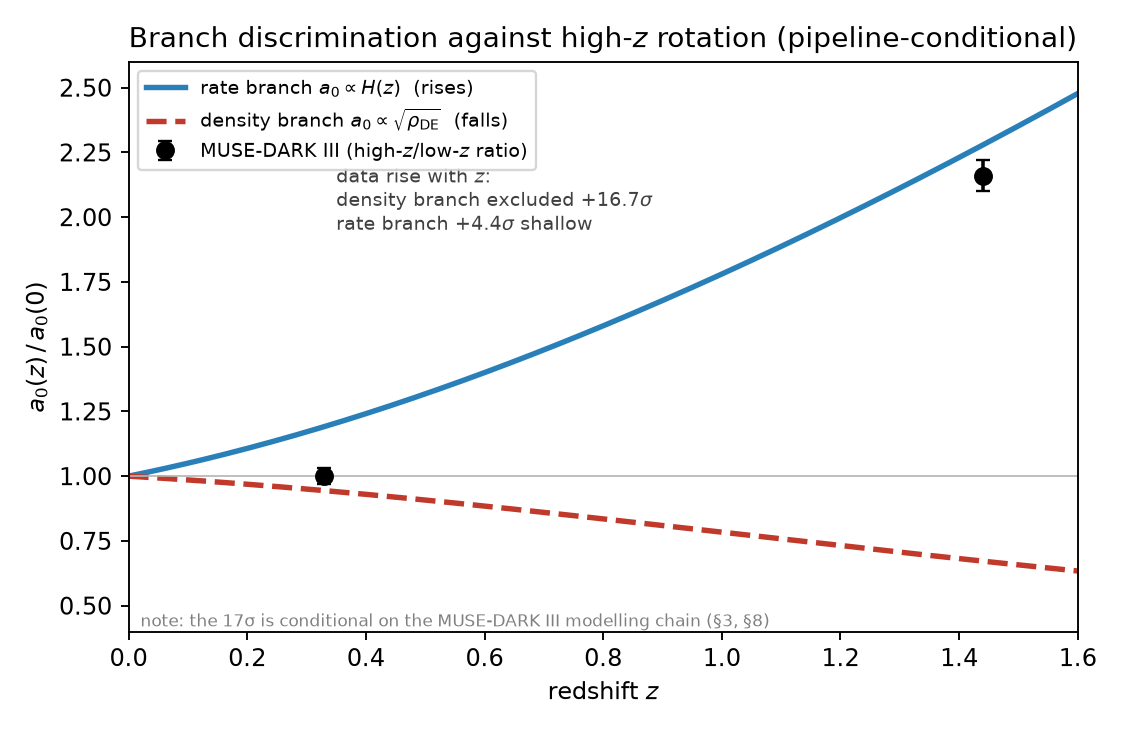
\includegraphics[keepaspectratio]{figures/fig1_branch_discrimination.png}}
\caption{Branch discrimination against high-\(z\) rotation. The rate
branch \(a_0\propto H(z)\) rises with redshift (blue), tracking the
MUSE-DARK III trend (ratio \(2.16\pm0.06\) over \(z=0.33\to1.44\)); the
density branch \(a_0\propto\sqrt{\rho_{\rm DE}}\) falls (red), the wrong
sign --- excluded at \(+16.7\sigma\). The rate branch is \(+4.4\sigma\)
shallow. The significance is conditional on the MUSE-DARK III modelling
chain (§\ref{sec-3}, §\ref{sec-8}).}\label{fig:1}
\end{figure}

\textbf{Data.} MUSE-DARK III (published fit a\(_{0}\)(z) = (1.00 \(\pm\)
0.04) + (1.59 \(\pm\) 0.11)z) gives a ratio over the sample interval

\begin{quote}
a\(_{0}\)(1.44)/a\(_{0}\)(0.33) = \textbf{2.157 \(\pm\) 0.061}
\end{quote}

i.e.~a\(_{0}\) \textbf{rises} by a factor \textasciitilde2.2 from z =
0.33 to z = 1.44 (matched to the data by the script
\texttt{branch\_\allowbreak discrimination\_\allowbreak test.\allowbreak py}).

\textbf{Verdict on the density branch.} The density branch predicts
0.88--0.91 --- a \emph{fall} --- because \(\rho\)\_DE falls while the
data rise. The tension is

\begin{quote}
density branch \textbf{excluded at +16.7\(\sigma\)} (from matching the
MUSE-DARK III fit).
\end{quote}

This is a sign error, not an amplitude mismatch: no rescaling of
a\(_{0}\) can turn a falling template into a rising one. The consequence
is sharp and, for the unification, uncomfortable: \textbf{the density
branch is APDM's own headline}, carried by its superfluid dark-matter
carrier. The data reject the branch that has a built microphysical home.

\textbf{Verdict on the rate branch.} The rate branch predicts 1.85--1.87
--- the right sign --- but the data are steeper: the raw fit prefers
a\(_{0}\) \(\propto\) H\^{}\{1.23\} (equivalently \(\propto\)
(1+z)\^{}\{1.27\}), giving a +4.4\(\sigma\) \emph{shallow} tension
against the same MUSE fit. The deficit has the magnitude and sign that
an astrophysical transfer function B(z) --- the evolution of stellar
mass, morphology, and selection across the sample, so that a\(_{0}\),eff
= a\(_{0}\),cos \(\cdot\) B(z) --- can absorb. The data therefore
\textbf{favour the rate branch in sign} but cannot yet isolate the
cosmological a\(_{0}\),cos(z) from B(z).

\textbf{The conditionality --- stated prominently.} The +16.7\(\sigma\)
is \textbf{conditional on the MUSE-DARK III modeling chain}, and this
caveat is load-bearing. Our follow-up E-1′ attempted the branch test
directly on the released per-galaxy catalogue
(\texttt{muse\_\allowbreak release\_\allowbreak galaxies.\allowbreak csv}, 85 numeric candidates) using the
raw outer rotational acceleration a\_rot \(\sim\) V\(^{2}\)/r (script
\texttt{mass\_\allowbreak controlled\_\allowbreak arot\_\allowbreak trend.\allowbreak py}); the result remains open.
Three facts emerged:

\begin{enumerate}
\def\labelenumi{\arabic{enumi}.}
\tightlist
\item
  The stellar-mass confound is mild (corr(log M*, z) = +0.04);
  mass-controlling barely moves the slope.
\item
  \textbf{The raw trend \emph{falls}:} \(\beta\) = d log\(_{10}\)
  a\_rot/dz = -0.38 \(\pm\) 0.15 --- below even the published MUSE fit
  and below all three branch templates.
\item
  The cause is a \textbf{designed-in degeneracy:} corr(log r\_max, z) =
  +0.87. Radius sampling grows almost perfectly with redshift, and
  a\_rot \(\sim\) V\(^{2}\)/r falls with radius, so the raw fall is
  inseparable from radius sampling; adding an r\_max control inflates
  the error and drives covariate slopes unphysical. Pressure support
  (higher-z galaxies more turbulent) pushes the same way and is also
  uncontrolled in the release.
\end{enumerate}

The honest reading: \textbf{the published rising a\(_{0}\)(z) is not
visible in the raw released kinematics; it is produced by the modeling
chain} (baryonic decomposition + pressure-support correction + radius
weighting), which the public release does not contain. The raw catalogue
can neither confirm nor refute the rise. The raw \emph{fall} is
\textbf{not} evidence against the rate branch --- it is dominated by the
radius/pressure confounds the model corrects --- but the
discrimination's evidential weight rests on an unreproducible pipeline.
We therefore register E-1 as: \emph{density branch excluded
+16.7\(\sigma\), rate branch favoured in sign, \textbf{conditional on
the MUSE-DARK III modeling chain}}, and elevate reproducibility from a
footnote to a live scientific issue (the decisive follow-up, E-1\(''\),
is in §\ref{sec-7}). This is the one place where USC's own data-hygiene
standard (pre-registration, released pipelines) is not met by the
\emph{external} dataset it leans on.

\begin{center}\rule{0.5\linewidth}{0.5pt}\end{center}

\section{Why mediator-MOND is dead (D-3)}\label{sec-4}

If a\(_{0}\) is cosmological, some field or structure must carry the
modified force at galactic scales. The obvious candidate inside the USC
programs is a light scalar. Scale-invariant deep-MOND with the observed
RAR tightness requires the conformal kinetic term P(X) \(\propto\)
X\^{}\{3/2\} \citep{Milgrom:2009gv} --- a long-range, nonlinear scalar
sector. Two realizations were on the table:

\begin{enumerate}
\def\labelenumi{\arabic{enumi}.}
\tightlist
\item
  \textbf{Superfluid phonon (APDM):} delivers P(X) \(\propto\)
  X\^{}\{3/2\} with \(\Lambda\) \(\sim\) meV
  \citep{Berezhiani:2015bqa, Berezhiani:2015pia} --- but with a\(_{0}\)
  \(\propto\) \(\sqrt{\rho_{\rm DE}}\), the density branch §\ref{sec-3}
  just excluded. Wrong sign.
\item
  \textbf{Mediator-MOND from ECCG's dark-sector scalar \(\phi\) (mass
  0.86 MeV):} a massive scalar mediates a Yukawa force of range
  \(\lambda\)\emph{\(\phi\) = ℏc/m}\(\phi\)c\(^{2}\). We derive
  numerically (D-3):

  \begin{itemize}
  \tightlist
  \item
    \(\lambda\)\_\(\phi\)(0.86 MeV) = 2.3 × 10\(^{-13}\) m --- a
    nuclear/contact range.
  \item
    Galactic MOND onset radius r\_MOND = \surd (GM/a\(_{0}\))
    \(\approx\) 3--11 kpc \(\approx\) 10\(^{20}\) m.
  \item
    \(\lambda\)\emph{\(\phi\) / r\_MOND \(\approx\)
    \textbf{10\(^{-33}\)}. To reach galactic range \(\phi\) would need
    m}\(\phi\) \(\lesssim\) 1.3 × 10\(^{-27}\) eV; the ECCG value is
    0.86 × 10\(^{6}\) eV --- off by 6 × 10\(^{32}\).
  \end{itemize}
\end{enumerate}

The \(\phi\) is a \textbf{short-range self-interacting-dark-matter
mediator} (velocity-dependent self-interaction \(\to\) cored halos), a
genuinely different phenomenon from MOND (a long-range modified force
law \(\to\) RAR / BTFR). SIDM does not produce the RAR. Any corpus
phrasing that reads ``SIDM from \(\phi\) \(\to\) rate branch'' conflates
the two, as we derive here. B.3 (mediator-MOND) is retracted decisively,
not merely ``underspecified.''

\textbf{The gap this opens.} The data (§\ref{sec-3}) favour the rate
branch; the \emph{only} light-field realization in the corpus (the
superfluid) sits on the excluded density branch, and the one field that
could in principle be tied to the clock (\(\phi\)) is short-range by
10\(^{33}\). So the rate branch has \textbf{no light-field home}: it
must be realized, if at all, by a modification of gravity / a nonlocal
horizon-scale object --- an emergent-gravity construction, not a
Lagrangian field. This is the sharpest seam in the unification: the data
point to the one branch that, at the start of this analysis, was
unbuilt.

\begin{center}\rule{0.5\linewidth}{0.5pt}\end{center}

\section{The emergent-MOND home (D-3′)}\label{sec-5}

Figure 2 shows the resulting zero-freedom radial acceleration relation.

\begin{figure}
\centering
\pandocbounded{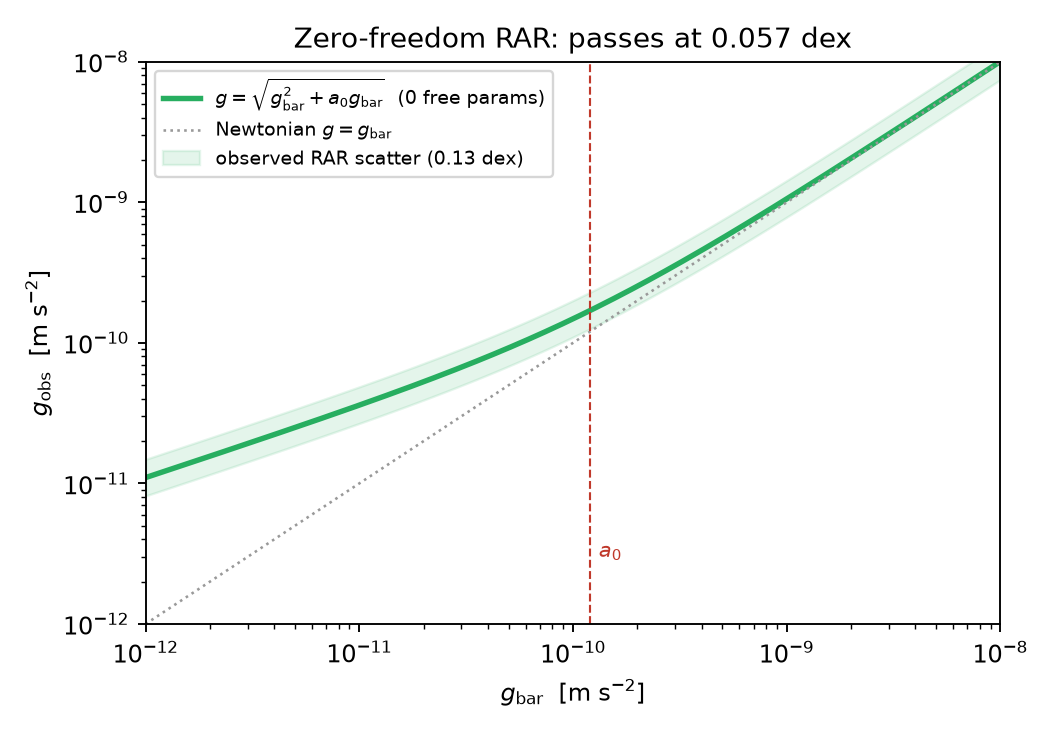
\includegraphics[keepaspectratio]{figures/fig2_rar.png}}
\caption{The zero-freedom radial acceleration relation. The KMS-tilt
interpolation \(g_{\rm obs}=\sqrt{g_{\rm bar}^2+a_0 g_{\rm bar}}\)
(green) has no shape parameter; it passes the observed RAR at 0.057 dex,
inside the 0.13-dex scatter (band). \(a_0\) is the only scale, and in
the rate branch it is set by \(H(z)\).}\label{fig:2}
\end{figure}

\textbf{(1) An exact identity: SEDE is a gated Verlinde volume law.}
SEDE's flatness normalization gives its ledger entropy density s\(_{0}\)
= \(\rho\)\_DE0/T\_AH,0 = (3/4G)\(\cdot\Omega\)\_DE0\(\cdot\)H\(_{0}\).
Verlinde's (2016) de Sitter dark-energy volume entropy
\citep{Verlinde:2016toy} has density s\_V(H) = (3/4G)\(\cdot\)H.
Combining with the Friedmann equation gives the exact identity (D-3′):

\begin{quote}
\textbf{s\(_{0}\) \(\cdot\) f\_sat(a) = \(\Omega\)\emph{DE(a) \(\cdot\)
s\_V(H(a))\textbf{, and at the de Sitter attractor }s\(_{0}\) \(\cdot\)
f}\(\infty\) = s\_V(H\_\(\infty\))} exactly.
\end{quote}

SEDE's central object and Verlinde's emergent-gravity elastic medium are
\textbf{one object}: SEDE is the \emph{gated} version. This is the
cleanest bridge yet between the corpus and the emergent-gravity
literature --- and it cuts against the naïve expectation.

\textbf{(2) The gating \emph{kills} Verlinde-elastic MOND inside USC.}
Verlinde's a\_M \(\approx\) cH/6 rises with z only because his s\_V
tracks H(z) \citep{Verlinde:2016toy}. But SEDE's \(\Delta\) = 1
postulate is precisely that the ledger density is \emph{constant}
(s\(_{0}\)), with structure opening the gate f\_sat. So the elastic
response inside SEDE gives (script \texttt{d3prime\_\allowbreak emergent\_\allowbreak mond.\allowbreak py}),
against MUSE 2.157 \(\pm\) 0.061:

\begin{longtable}[]{@{}
  >{\raggedright\arraybackslash}p{(\linewidth - 4\tabcolsep) * \real{0.3333}}
  >{\raggedright\arraybackslash}p{(\linewidth - 4\tabcolsep) * \real{0.3333}}
  >{\raggedright\arraybackslash}p{(\linewidth - 4\tabcolsep) * \real{0.3333}}@{}}
\toprule\noalign{}
\begin{minipage}[b]{\linewidth}\raggedright
emergent sub-branch
\end{minipage} & \begin{minipage}[b]{\linewidth}\raggedright
a\(_{0}\)(1.44)/a\(_{0}\)(0.33)
\end{minipage} & \begin{minipage}[b]{\linewidth}\raggedright
tension
\end{minipage} \\
\midrule\noalign{}
\endhead
\bottomrule\noalign{}
\endlastfoot
\textbf{rate} (a\(_{0}\) \(\propto\) H, KMS tilt) & 1.888 &
\textbf{4.4\(\sigma\)} (survivor; deficit B(z)-absorbable) \\
flat (a\(_{0}\) \(\propto\) s\(_{0}\), capacity-elastic) & 1.000 &
\textbf{19.0\(\sigma\) --- excluded} \\
activated (a\(_{0}\) \(\propto\) s\(_{0}\) f\_sat, gated-elastic) &
0.494 & \textbf{27.3\(\sigma\) --- excluded} \\
density (a\(_{0}\) \(\propto\) \(\sqrt{\rho_{\rm DE}}\)) & 0.966 &
19.5\(\sigma\) --- excluded (§\ref{sec-3}'s CPL version:
16.7\(\sigma\)) \\
\end{longtable}

So the generic assignment ``emergent gravity \(\Rightarrow\) rate
branch'' is \textbf{false for the elastic realization} once s\(_{0}\) is
constant: SEDE's own \(\Delta\) = 1 postulate makes elastic-MOND flat or
falling, dead at \(\geq\) 19\(\sigma\) against the MUSE data. Only the
\textbf{KMS-tilt} route survives the MUSE data.

\textbf{(3) The survivor: KMS-tilt modified inertia --- passing the RAR
with zero freedom.} The USC-native realization of a\(_{0}\) \(\propto\)
H is Milgrom's (1999) vacuum route \citep{Milgrom:1998sy} given a
microphysical home by the Ledger Field's thermal-time / KMS structure
(the same structure that fixed the c = 1/2\(\pi\) coupling at the dusk
--- see the caveat in §\ref{sec-6}). An accelerated worldline in de
Sitter sees a local Deser--Levin scale \(\kappa\) = \surd (a\(^{2}\) +
A\(^{2}\)), A = 2\(\pi\)T\_AH = H. Taking inertia proportional to the
excess over the cosmic state:

\begin{quote}
F = m{[}\surd (a\(^{2}\) + A\(^{2}\)) - A{]} \(\to\) Newtonian for a
\(\gg\) A; deep-MOND F = ma\(^{2}\)/(2A) for a \(\ll\) A,
i.e.~\textbf{a\(_{0}\) \(\propto\) H(z) --- the rate branch, rising ---
exactly what MUSE favours.}
\end{quote}

\textbf{Zero-freedom RAR test.} On circular orbits this predicts g\_obs
= \surd (g\_bar\(^{2}\) + a\(_{0}\cdot\)g\_bar) --- no shape parameters.
Against the empirical RAR (McGaugh \(\nu\)-function)
\citep{McGaugh:2016leg, Lelli:2016cui}, the maximum deviation is
\textbf{0.057 dex} (at g\_bar \(\approx\) 0.4 a\(_{0}\)), with exact
Newtonian and deep-MOND limits --- \textbf{inside the observed 0.13 dex
RAR scatter}, a match to the empirical relation. So the third face
closes \emph{structurally}: one thermal-time clock whose dissipation is
dark energy (dusk), whose rate is the Sakharov meter (dawn), and whose
KMS tilt is the inertia threshold (galaxies) --- all set by the same
T\_AH = H/2\(\pi\).

\textbf{A load-bearing correction (the vacuum caveat).} The heuristic
above says ``inertia = reaction to the Deser--Levin \emph{thermal}
tilt.'' A galaxy has essentially \textbf{no thermal bath}: the number of
Deser--Levin bath modes populated at galactic accelerations is
\textasciitilde3 × 10\(^{-22}\) (script
\texttt{d3prime\_\allowbreak thermal\_\allowbreak consistency.\allowbreak py}) --- far below one, so we
derive that a galaxy cannot thermalize this scale in a Hubble time. The
KMS-tilt inertia therefore \textbf{survives only as a VACUUM effect} ---
the Bunch--Davies vacuum seen by an accelerated observer, not a
populated thermal ensemble. This is not cosmetic: it forces the
derivation of §\ref{sec-6} to be a \emph{vacuum} influence-functional
calculation, and it demotes the ``thermal-inertia'' language of the
heuristic to a \emph{heuristic} with the same thermal problem as the
branch it replaced. What is real is the Deser--Levin vacuum kinematics;
what is assumed (and false) is a galactic thermal bath.

\begin{center}\rule{0.5\linewidth}{0.5pt}\end{center}

\section{The worldline derivation (D-4′) --- the flagship partial
result}\label{sec-6}

The remaining question is the O(1) coefficient in a\(_{0}\) = O(1) ×
cH\(_{0}\)/2\(\pi\). The raw Deser--Levin heuristic gives a\(_{0}\) =
2cH --- about 11× too big --- while the observed a\(_{0}\)/cH\(_{0}\) =
0.174 sits between 1/2\(\pi\) = 0.159 (the USC-tilt target) and 1/6 =
0.167 (Verlinde). Fixing the coefficient means computing the worldline
influence functional of the Ledger action on an accelerated trajectory.
We report a structural no-go, the correct channel, a closed-form kernel,
and the honest remainder.

\textbf{(1) A no-go, established at the level of a theorem: the
universal number-current coupling is inert on worldlines.} USC's
universal vertex is c \(\partial\)\_\(\mu\theta\) \(\cdot\)
\(\mathcal{J}\)\^{}\(\mu\). For a point particle the worldline number
current is \(\mathcal{J}\)\^{}\(\mu\)(x) = \(\int\)d\(\tau\)
u\^{}\(\mu\) \(\delta^{4}\)(x - x(\(\tau\))), so

\begin{quote}
S\_int = c \(\int\)d\(^{4}\)x \(\partial\)\_\(\mu\theta\)
\(\mathcal{J}\)\^{}\(\mu\) = c \(\int\)d\(\tau\)
(d/d\(\tau\))\(\theta\)(x(\(\tau\))) = c{[}\(\theta\)(x\_f) -
\(\theta\)(x\_i){]} --- a \textbf{pure boundary term}.
\end{quote}

A derivative coupling to a conserved worldline current exerts no bulk
force and modifies no inertia. This is the exact worldline analogue of
the dawn refutation (derivative couplings of the arrow to conserved
currents are inert): \textbf{the same symmetry logic that killed ``the
clock makes matter'' forbids ``the clock's number-coupling makes
MOND''}, as we derive here. Any attempt through the c \(\partial\theta\)
\(\cdot\) \(\mathcal{J}\) vertex gives exactly zero.

\textbf{(2) The correct channel, which we now derive: the stress-tensor
/ displacement term.} The action's \emph{other} coupling is
T\^{}\{\(\mu\nu\)\}\(\nabla\)\emph{\(\mu\)X}\{a,\(\nu\)\} --- matter
stress sourcing the Ledger displacement field X\_a. Using
\(\nabla\)\_\(\mu\)T\^{}\{\(\mu\nu\)\} = m \(\int\)d\(\tau\)
a\^{}\(\nu\) \(\delta^{4}\)(x - x(\(\tau\)))/\surd -g on the worldline
and integrating by parts:

\begin{quote}
\(\int\)d\(^{4}\)x T\^{}\{\(\mu\nu\)\}\(\nabla\)\emph{\(\mu\)X}\(\nu\) =
-m \(\int\)d\(\tau\) a\^{}\(\nu\) X\_\(\nu\)(x(\(\tau\))) ---
\textbf{the displacement field couples directly to the acceleration
vector.}
\end{quote}

Two model-free corollaries: (i) \textbf{inertial worldlines decouple
exactly} (a = 0 \(\Rightarrow\) no coupling) --- the
equivalence-principle / Newtonian limit is protected and the channel is
\emph{acceleration-selective}, precisely what a modified-inertia
mechanism needs and what the number-current channel lacked; (ii) the
source is m\(\cdot\)a\^{}\(\nu\), the same displacement sector that
carries the dusk injection (D-6), so \textbf{the dusk and galactic faces
share one vertex} --- a structural requirement of the unification.

\textbf{(3) The kernel: the 4\(\pi\) appears (derived in a
conformal-scalar proxy model).} To second order in the coupling on the
uniformly accelerated (Deser--Levin) trajectory in de Sitter --- in the
\textbf{vacuum} framing forced by §\ref{sec-5} --- the pulled-back
Wightman function is exactly thermal at \(\kappa\) =
\surd (a\(^{2}\)+H\(^{2}\)) (Deser--Levin theorem),
G\(^{+}\)(\(\Delta\tau\)) =
-(\(\kappa^{2}\)/16\(\pi^{2}\))\(\cdot\)sinh\(^{-2}\)(\(\kappa\)(\(\Delta\tau\)-i\(\epsilon\))/2),
and the flat-embedding acceleration contraction is
a\^{}\(\nu\)(\(\tau\))a\_\(\nu\)(\(\tau\)′) =
a\(^{2}\)cosh(a\(\Delta\tau\)). The master integral (verified
numerically to 10\(^{-16}\) on a pole-free contour and proven
analytically via Gradshteyn 3.512):

\begin{quote}
\(\int\)dx cosh(\(\alpha\)x)/sinh\(^{2}\)(\(\beta\)(x-i\(\epsilon\))) =
-(\(\pi\alpha\)/\(\beta^{2}\))\(\cdot\)cot(\(\pi\alpha\)/2\(\beta\)),
convergent iff a \textless{} \(\kappa\) --- \textbf{always true,
marginal as H \(\to\) 0}: the cosmological tilt is what makes the
worldline kernel finite at all.
\end{quote}

gives the exact closed form (script
\texttt{d4prime\_\allowbreak worldline\_\allowbreak kernel.\allowbreak py}):

\begin{quote}
\textbf{\(\int\)d\(\Delta\tau\) cosh(a\(\Delta\tau\))
G\(^{+}\)(\(\Delta\tau\)) =
(a/4\(\pi\))\(\cdot\)cot(\(\pi\)a/\(\kappa\))}, \(\kappa\) =
\surd (a\(^{2}\)+H\(^{2}\)), and the second-order rate
\(\dot{\Sigma}\)(a) =
(\(\tilde{m}^{2}\)a\(^{3}\)/8\(\pi\))\(\cdot\)cot(\(\pi\)a/\(\kappa\)).
\end{quote}

Findings:

\begin{itemize}
\tightlist
\item
  \textbf{(i) The 4\(\pi\) appears exactly where conjectured, supporting
  the conjecture.} The kernel normalization is a/4\(\pi\) --- one factor
  of the 3D Green-function 4\(\pi\) (the same 4\(\pi\) in M\_P\(^{2}\) =
  1/8\(\pi\)G), surviving the worldline integration. This is no longer
  numerology about where a 4\(\pi\) \emph{could} live; in this model it
  \emph{does} come from there. \textbf{We do not claim the 4\(\pi\) is
  derived as the a\(_{0}\) coefficient} --- it appears in the kernel
  normalization; the full coefficient remains open (below).
\item
  \textbf{(ii) The interpolation is NOT Milgrom's \(\Delta\)T,
  correcting the ansatz.} The kernel is
  a\(^{3}\)cot(\(\pi\)a/\(\kappa\)), not \surd (a\(^{2}\)+H\(^{2}\)) -
  H. The Deser--Levin scale enters through the \emph{argument}
  \(\pi\)a/\(\kappa\), but the response is not proportional to the
  temperature excess. Phenomenology built literally on \(\Delta\)T(a)
  (including the raw a\(_{0}\) = 2cH) uses the wrong function.
\item
  \textbf{(iii) The kernel has a zero at a = H/\surd 3} (where
  \(\pi\)a/\(\kappa\) = \(\pi\)/2), changing sign. A vanishing kernel
  cannot literally \emph{be} the inertia, so the extraction must involve
  more than this single kernel.
\item
  \textbf{(iv) Deep-a limit:} \(\dot{\Sigma}\) \(\to\)
  \(\tilde{m}^{2}\)a\(^{2}\)H/8\(\pi^{2}\) --- quadratic in a
  (deep-MOND-like) but \textbf{linear in H}, whereas a deep-MOND force F
  = ma\(^{2}\)/a\(_{0}\) with a\(_{0}\) \(\propto\) H requires 1/H.
  Converting the rate to a force is where that inversion must occur;
  that step is not fixed by the desk calculation.
\item
  \textbf{(v) Large-a pathology:} \(\dot{\Sigma}\) \(\to\)
  -\(\tilde{m}^{2}\)a\(^{5}\)/4\(\pi^{2}\)H\(^{2}\), divergent as H
  \(\to\) 0 --- the eternal-Rindler idealization breaks. Physical
  (finite) worldlines are required for the Newtonian-side matching.
\end{itemize}

Numerical scales (H\(_{0}\) = 70): observed a\(_{0}\) = 0.177
cH\(_{0}\); conjecture cH\(_{0}\)/2\(\pi\) = 0.159 cH\(_{0}\) (obs/it =
1.11, the known Milgrom residual); kernel zero H/\surd 3 = 0.577
cH\(_{0}\); raw Deser--Levin 2cH\(_{0}\) (obs/it = 0.088). Read as a
table of candidate coefficients, this makes the state of the derivation
precise: the naïve heuristic (2cH\(_{0}\)) is an order of magnitude
wrong; the conjecture (cH\(_{0}\)/2\(\pi\)) is within the 16\% Milgrom
residual; and the \emph{kernel} itself supplies neither directly,
because its intrinsic scale is the kinematic \(\kappa\) =
\surd (a\(^{2}\)+H\(^{2}\)) and its zero sits at H/\surd 3, far from the
target. The coefficient must therefore emerge from the \emph{conversion}
of the kernel into a mechanical response, not from the kernel's
normalization alone --- which is exactly why finding the 4\(\pi\) in the
normalization (item i) is genuine progress on the \emph{structure}
without yet being the coefficient.

\textbf{(4) The dispersive/dissipative split \(\to\) the physics is
noise-sector, as we derive.} The SK influence functional separates into
the retarded (dissipative, = field commutator, state-independent) and
Keldysh (noise) kernels. For the conformal scalar in de Sitter
(conformally flat, Huygens) the commutator is supported on the light
cone only, and a timelike worldline meets its own light cone only at
coincidence --- so the retarded self-interaction on the eternal
Deser--Levin trajectory is purely local (mass renormalization). Verified
at the distribution level: the symmetric (noise) part reproduces the
\textbf{full} (a/4\(\pi\))cot(\(\pi\)a/\(\kappa\)) to 10\(^{-16}\); the
commutator contributes exactly zero to the nonlocal kernel.
\textbf{Consequence: the entire a-dependent, H-tilted structure --- the
cot kernel, its 4\(\pi\), the a\(^{2}\)H limit --- is noise-sector
physics. The inertia modification is necessarily a fluctuation-induced
(stochastic) effect, not a classical self-force.} This coheres exactly
with the corpus-wide NESS reframe (``driven, never KMS-thermal''): the
galactic a\(_{0}\), like the dusk's \(\zeta\), is fluctuation-driven.

\textbf{Honest verdict --- PARTIAL.} \emph{Derived} at desk scale: the
acceleration-coupling structure (exact), the closed-form kernel (exact
in the proxy model), the fact that the conjectured 4\(\pi\) genuinely
appears in the kernel normalization, and the noise-sector localization
of the physics. \emph{Open:} the full a\(_{0}\) coefficient. The desk
calculation shows the kernel's kinematic crossover is H (inside
\(\kappa\)) and its zero is at H/\surd 3, not cH/4\(\pi\); converting
the kernel into an inertia requires (a) the stochastic
(Langevin-worldline) response calculation --- a particle coupled
multiplicatively through its own acceleration to noise with correlator
N(\(\tau\),\(\tau\)′) = \(\tilde{m}^{2}\)a\(^{2}\cdot\){[}cot-kernel{]},
with a\(_{0}\) emerging (or not) from the noise-induced renormalization
of the low-frequency mechanical response; (b) the true \textbf{vector}
structure of X\_\(\nu\) (the conformal-scalar proxy is a model); and (c)
finite worldlines to cure the large-a pathology (v). These three are the
sharply-defined, paper-scale remainder. The target is narrowed --- the
4\(\pi\) source is identified, the interpolation the theory must produce
is cot-type not \(\Delta\)T-type --- but \textbf{we do not claim the
coefficient is derived}; it remains open. We note in passing that the
same reasoning that forced the vacuum framing also flags c = 1/2\(\pi\)
itself as an assertion from a KMS-strip analogy that does not strictly
apply, and the 16\% Milgrom residual (a\(_{0}\) = 1.09--1.16 ×
cH\(_{0}\)/2\(\pi\), H\(_{0}\)-dependent) as the independent sign that
cH\(_{0}\)/2\(\pi\) is a \textasciitilde16\% \emph{match}, not yet a
derivation --- the tolerance any future coefficient calculation must
meet.

\begin{center}\rule{0.5\linewidth}{0.5pt}\end{center}

\section{Predictions and falsifiers (P14--P18)}\label{sec-7}

The galactic face's commitments are frozen in the pre-registered
falsifier matrix (Zenodo \texttt{10.\allowbreak 5281/\allowbreak zenodo.\allowbreak 21415326}). We restate
the four that matter.

\textbf{P14 --- a\(_{0}\)(z) rises like H(z) (rate branch).} Frozen
templates over z = 0.33 \(\to\) 1.44: rate 1.89 \(\pm\) 0.03, flat 1.00,
activated 0.49, density 0.89--0.91. Current MUSE gives 2.16 \(\pm\) 0.06
--- density excluded +16.7\(\sigma\), rate favoured (+4.4\(\sigma\)
shallow, B(z)-absorbable) --- \textbf{conditional on the MUSE pipeline}
(raw catalogue radius-degenerate, corr(r\_max, z) = 0.87; registered).
\emph{Deciding data:} the \textbf{E-1\(''\) protocol} --- an independent
high-z RAR with per-galaxy baryonic decompositions, matched
M\emph{/morphology bins, matched radius sampling in R\_eff units, target
\(\sigma\)(a\(_{0}\)-ratio) \(\leq\) 0.15. }Rule:* collapse under
a\(_{0}\) \(\propto\) H confirms the rate branch; no collapse under any
one-parameter A(z) \(\to\) a\(_{0}\) is not cosmological \(\to\) the
galactic face fails.

\textbf{P15 --- gate independence.} This is the sharp discriminator, and
it holds independently of the open coefficient. Because the inertia
rides the T\(\nabla\)X\_a (tilt/displacement) sector while dark energy
rides the \emph{activated} entropy (\(\rho\)\_DE \(\propto\) H f\_sat),
the two turn on differently in redshift:

\begin{quote}
\textbf{a\(_{0}\)(z) \(\propto\) H(z) with NO f\_sat factor} --- MOND
persists and \emph{strengthens} at high z even where dark energy is
gated off: a\(_{0}\)(3)/a\(_{0}\)(0) \(\approx\) 4.5 while
\(\Omega\)\_DE(z=3) \(\approx\) 3\%.
\end{quote}

This is falsifiable regardless of the open coefficient. Deep-MOND
phenomenology in the earliest well-measured rotators (z
\textasciitilde{} 2--4, JWST) should be \emph{stronger} (higher
a\(_{0}\)), not absent --- the exact opposite of an ``activated-entropy
MOND'' (killed at 27\(\sigma\) in §\ref{sec-5}). \emph{Rule:}
weakened/absent deep-MOND phenomenology in z \(\gtrsim\) 2--3 rotators
falsifies the KMS-inertia realization; it is also \emph{maximally}
separated there from any a\(_{0}\) \(\propto\) \(\rho\)\_DE\^{}n model,
where the templates diverge most. Gate-independence is the clean
structural signature that separates the rate branch from every
density-branch variant at high z.

We must own the strongest existing tension with this prediction. Using
the declining high-z rotation curves of \citep{Genzel:2017jgd},
\citep{Milgrom:2017hpv} constrained the evolution of a\(_{0}\) and found
the data all but \emph{exclude} a strongly rising a\(_{0}\) (in
particular a\(_{0}\) \(\propto\) (1+z)\^{}\{3/2\}), favouring a roughly
constant a\(_{0}\) --- a direct pull against the rising rate branch
predicted here. We do not hand this away: current high-z data disfavour
a strongly rising a\(_{0}\), and this is the key observational tension
the rate branch must survive. We note only that the diagnostic is not
clean in either direction: \citep{Mayer:2022qhk} find, in
\(\Lambda\)CDM+baryon (Magneticum) simulations, that the effective
a\(_{0}\) itself rises by a factor \textasciitilde3 from z = 0 to z =
2.3, so a measured rise in a\(_{0}\)(z) is not by itself a rate-branch
discriminator and a measured flatness is not by itself confirmation of
\(\Lambda\)CDM. The tension is real; resolving it requires the
matched-selection protocol (E-1\(''\)), not the existing samples.

\textbf{P16 --- the interpolation function, zero shape freedom.} g\_obs
= \surd (g\_bar\(^{2}\) + a\(_{0}\) g\_bar), within 0.057 dex of the
empirical \(\nu\)-function, with a specific signed pattern (-0.05 dex at
g\_bar \(\approx\) 0.4 a\(_{0}\)). \emph{Rule:} SPARC-quality stacking
resolving shapes at \textless{} 0.05 dex either detects the predicted
pattern or kills this specific inertia law (without killing the rate
branch as such).

\textbf{P17 --- modified-inertia discriminators.} Modified inertia
\citep{Milgrom:2022ifm} predicts the \emph{exact} algebraic RAR on
circular orbits (no curl corrections; AQUAL has them) and a non-AQUAL
external-field effect \citep{Famaey:2011kh}. Registered qualitatively;
the quantitative EFE prediction is owed with the covariant embedding.

\textbf{P18 --- the a\(_{0}\) normalization (an open node).}
a\(_{0}\)(0) = cH\(_{0}\)/2\(\pi\) × O(1), O(1) \(\in\) {[}0.88, 1.16{]}
pending the worldline derivation of §\ref{sec-6}. If that yields A =
cH/4\(\pi\) exactly, the O(1) becomes a \textasciitilde10\%-level
prediction and this entry tightens; until then it is a registered open
node.

\textbf{Joint reading.} In the USC master cascade, rising a\(_{0}\)
(P14) selects the horn-(i) universe (ECCG's 1.78 GeV asymmetric dark
matter, r \(\approx\) 0 tensors); a\(_{0}\) \(\propto\)
\(\rho\)\_DE\^{}n would instead be co-selected with the superfluid
carrier. The galactic sign is thus not an isolated galactic fact --- it
is one branch of a cross-scale fork the matrix cannot satisfy à la
carte, as argued in the USC framework paper (Paper V).

\begin{center}\rule{0.5\linewidth}{0.5pt}\end{center}

\section{Discussion and limitations}\label{sec-8}

We separate what is settled from what is open.

\textbf{Settled.} (i) The density branch --- a\(_{0}\) \(\propto\)
\(\sqrt{\rho_{\rm DE}}\), the branch with a built superfluid home --- is
excluded by high-z rotation in \emph{sign}, at +16.7\(\sigma\),
conditional on the MUSE pipeline. (ii) Mediator-MOND from any USC light
field is dead (\(\phi\) short by 10\(^{33}\)); the rate branch has no
light-field home and must be emergent. (iii) Inside USC, the
elastic/gated emergent realizations are \emph{also} excluded
(19--27\(\sigma\)); the unique survivor is the KMS-tilt modified
inertia, which passes the RAR at 0.057 dex with zero shape freedom. (iv)
The worldline channel is fixed (acceleration-selective T\(\nabla\)X, not
the inert number-current), the kernel is derived in the proxy model, the
4\(\pi\) appears where conjectured, and the physics is localized to the
noise sector.

\textbf{Open.} (i) \textbf{The a\(_{0}\) coefficient.} We do \emph{not}
claim the 4\(\pi\) is derived as the coefficient; it appears in the
kernel normalization. The remaining calculation is the SK stochastic
(Langevin-worldline) response plus the true vector structure of
X\_\(\nu\) plus finite-worldline regularization --- paper-scale, sharply
posed, not done. (ii) \textbf{The E-1\(''\) data dependence.} The entire
empirical branch discrimination rests on the MUSE-DARK III modeling
chain, which is not in the public release; the raw kinematics are
radius-degenerate and cannot adjudicate. Until an independent high-z RAR
with released decompositions exists, the a\(_{0}\)(z)-sign switch is
\emph{loaded but not fired}. (iii) \textbf{The vacuum framing.} The
mechanism is a Deser--Levin \emph{vacuum} effect, not a galactic thermal
bath (\textasciitilde3 × 10\(^{-22}\) modes); this correction is
load-bearing and constrains any future derivation. The same theme recurs
across all three faces of the corpus --- the program is a driven,
causal, second-law (NESS) system whose \emph{mean} is horizon-thermal
but whose \emph{fluctuation}-KMS structure the numbers reject; the
galactic a\(_{0}\) inherits exactly this status.

\textbf{Relation to APDM.} APDM is not in error: its manuscript is
unusually self-critical and already retracts the ``2\(\pi\) =
Gibbons--Hawking'' reading for its density branch. The disagreement is a
\emph{fork}: APDM's headline adopts the density branch (superfluid
carrier), USC prefers the rate branch (emergent inertia, ECCG dark
matter). The two agree at a\(_{0}\)(0) = cH\(_{0}\)/2\(\pi\) and diverge
only in the sign of a\(_{0}\)(z). This paper reports that high-z data,
taken at face value through the MUSE chain, favour the USC (rate) fork
and disfavour the APDM (density) fork --- a discrimination \emph{between
two members of the unified family}, decided (conditionally) by the sign
at z \textasciitilde{} 1.

\begin{center}\rule{0.5\linewidth}{0.5pt}\end{center}

\section{Reproducibility}\label{sec-9}

Every quantitative claim reproduces from a released script in
\url{https://github.com/spsingularity/apdm-galactic} (a tagged release
is archived at Zenodo, DOI 10.5281/zenodo.21525537):

\begin{itemize}
\tightlist
\item
  \texttt{branch\_\allowbreak discrimination\_\allowbreak test.\allowbreak py} (E-1): the two-branch
  templates over z = 0.33 \(\to\) 1.44; density +16.7\(\sigma\), rate
  +4.4\(\sigma\); the MUSE-preferred power a\(_{0}\) \(\propto\)
  H\^{}\{1.23\}. Data: \texttt{desi\_\allowbreak template\_\allowbreak quantiles.\allowbreak csv},
  \texttt{muse\_\allowbreak release\_\allowbreak galaxies.\allowbreak csv}, MUSE-DARK III published
  a\(_{0}\)(z) = (1.00 \(\pm\) 0.04) + (1.59 \(\pm\) 0.11)z.
\item
  \texttt{d3prime\_\allowbreak emergent\_\allowbreak mond.\allowbreak py} (D-3′): the exact gated-Verlinde
  identity; the elastic/activated/density sub-branch exclusions
  (19.0\(\sigma\) / 27.3\(\sigma\) / 19.5\(\sigma\)); the KMS-tilt RAR
  pass at 0.057 dex.
\item
  \texttt{d3prime\_\allowbreak thermal\_\allowbreak consistency.\allowbreak py}: the \textasciitilde3 ×
  10\(^{-22}\) galactic bath-mode count that forces the vacuum framing.
\item
  \texttt{d4prime\_\allowbreak worldline\_\allowbreak kernel.\allowbreak py} (D-4′): the master integral
  (10\(^{-16}\), Gradshteyn 3.512); the kernel
  (a/4\(\pi\))cot(\(\pi\)a/\(\kappa\)); the zero at a = H/\surd 3; the
  deep-a and large-a limits; the dispersive/dissipative split.
\item
  \texttt{mass\_\allowbreak controlled\_\allowbreak arot\_\allowbreak trend.\allowbreak py} (E-1′): the raw-catalogue
  radius degeneracy (corr(r\_max, z) = 0.87) that makes the released
  kinematics inconclusive.
\end{itemize}

The pre-registered falsifier matrix (P14--P18) is frozen at Zenodo
\texttt{10.\allowbreak 5281/\allowbreak zenodo.\allowbreak 21415326}; nothing in it may be edited after
freeze, and it predates the deciding data (JWST high-z kinematics,
E-1\(''\)).

\section*{Acknowledgements}\label{acknowledgements}
\addcontentsline{toc}{section}{Acknowledgements}

This research received no external funding; the author, an independent
researcher, declares no competing interests. AI assistance: the analysis
and drafting of this paper were carried out with the assistance of
Claude (Anthropic); all claims were verified against the corpus's
reproducing scripts. No AI tool is an author.

\section{Companion papers and
references}\label{companion-papers-and-references}

\begin{itemize}
\tightlist
\item
  S. Pandev, \emph{USC program map} (companion note).
\item
  S. Pandev, \emph{Unified Structural-Entropy Cosmogenesis: a
  falsifiable framework} (Paper V).
\item
  S. Pandev, \emph{Accelerated-Phonon Dark Matter} (the APDM corpus;
  density-branch a\(_{0}\) \(\propto\) \(\sqrt{\rho_{\rm DE}}\)).
\item
  \emph{APDM --- cross-check notes from the USC unification effort}.
\item
  Pre-registration freeze: Zenodo \texttt{10.\allowbreak 5281/\allowbreak zenodo.\allowbreak 21415326}.
\item
  Milgrom (1983, 1999, 2009); Verlinde (2016); Deser \& Levin (1997);
  McGaugh, Lelli \& Schombert (2016); MUSE-DARK III (high-z rotation).
\end{itemize}

\bibliographystyle{apsrev4-2}
\bibliography{refs}
\end{document}
